\section{Additional Software Outputs}\label{sec:additional-outputs}


\subsection{Heatmap}

Figure \ref{fig:eye-heatmap}.

\begin{figure}
    \centering
    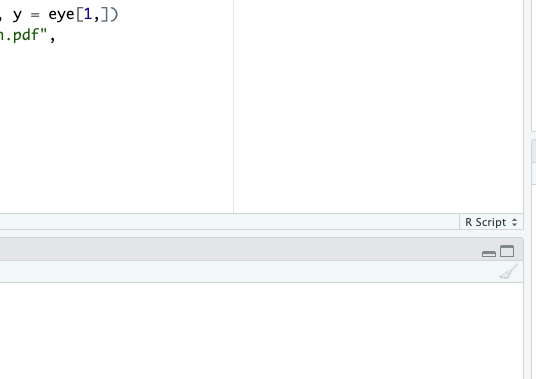
\includegraphics[width=0.75\linewidth]{figures/eye-heatmap.jpeg}
    \caption{Caption}
    \label{fig:eye-heatmap}
\end{figure}

\subsection{Additional Summary Plots}

Figure \ref{fig:additional-plots-01}.

\begin{figure}
    \centering
    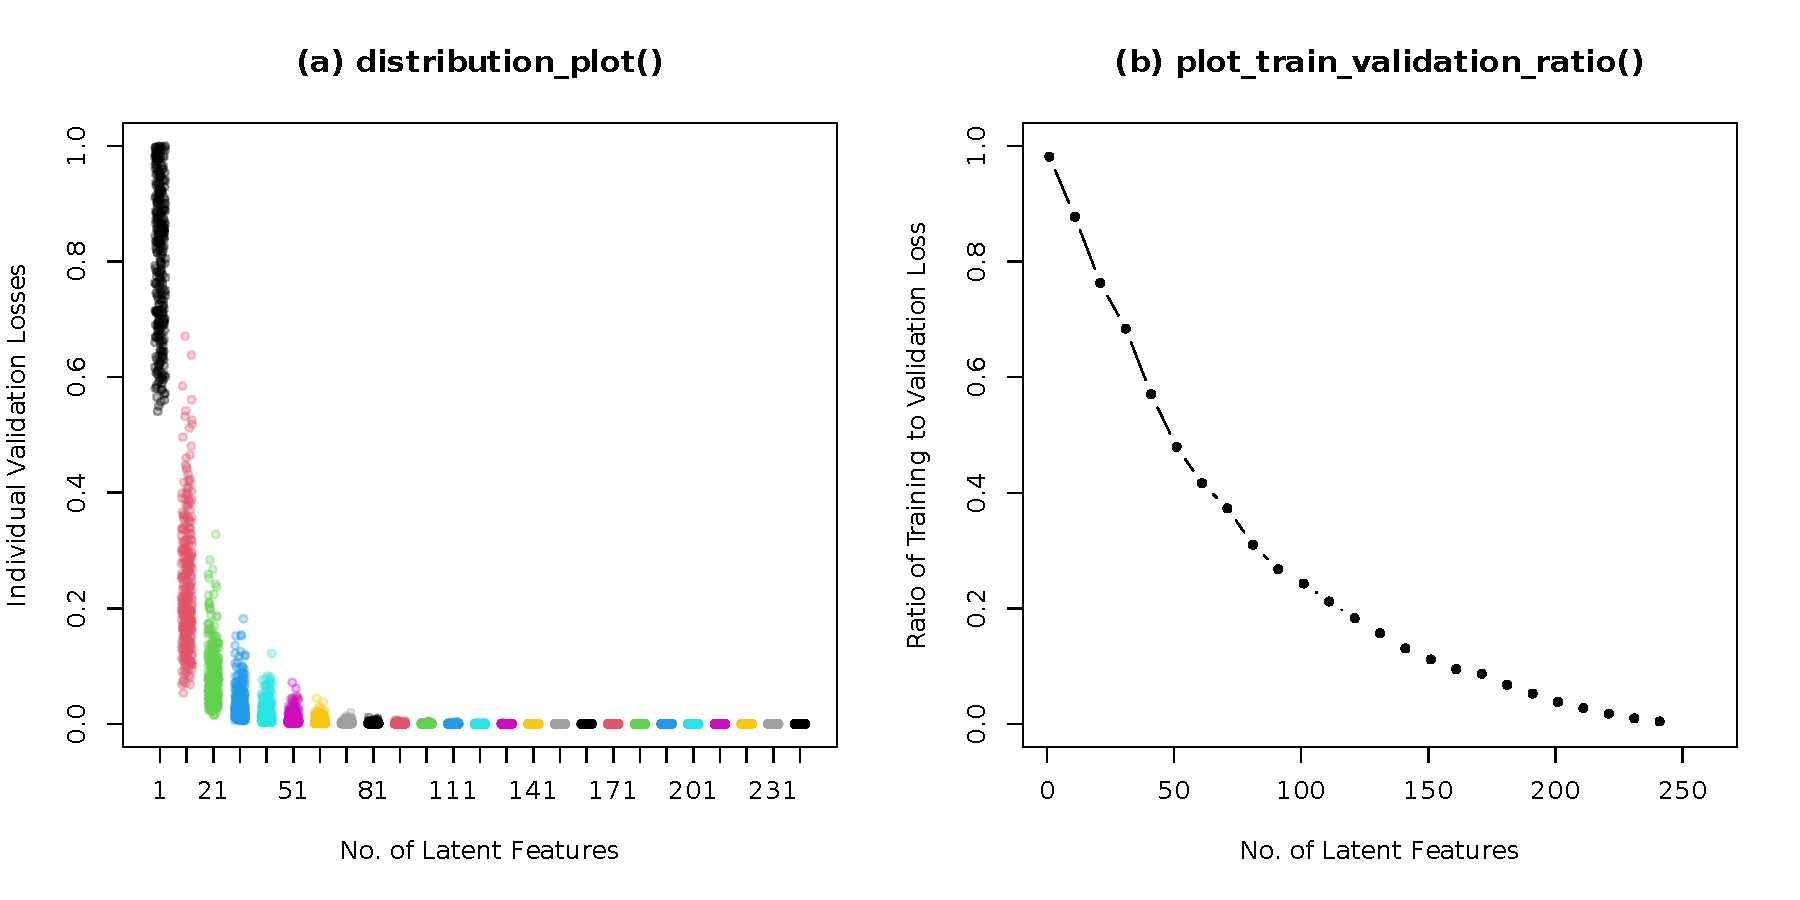
\includegraphics[width=1\linewidth]{figures/additional-plots-01.pdf}
    \caption{Additional wrapper functions that produce summary plots of \texttt{GLaRe()} outputs. \textbf{(a)} \texttt{distribution\_plot()} produces a dot-plot of the individual cross-validated information loss distribution. \textbf{(b)} \texttt{plot\_train\_validation\_ratio()} produces a point and line plot of the ratio of the total training and validation losses.
    Both plots are demonstrated on the Glaucoma dataset with a PCA representation from Section \ref{sec:software}.}
    \label{fig:additional-plots-01}
\end{figure}

\subsection{Reconstruction Plots}

Figure \ref{fig:eye-reconstruction}.

\begin{figure}
    \centering
    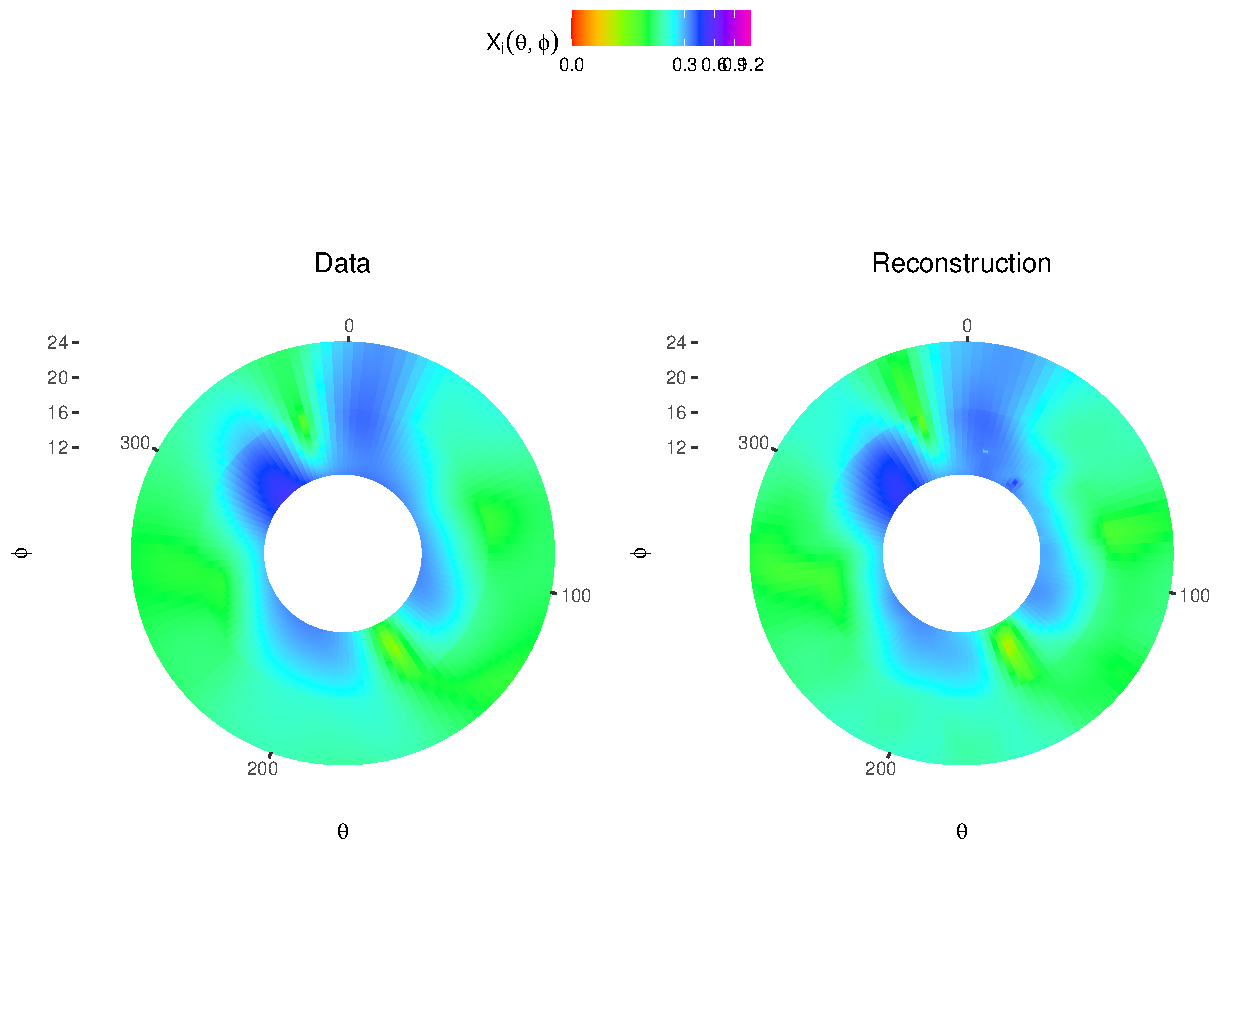
\includegraphics[width=0.75\linewidth]{figures/eye-reconstruction.pdf}
    \caption{Caption}
    \label{fig:eye-reconstruction}
\end{figure}